\begin{pastexam}[label={px:ncku-111-prog-10}]{成大資訊聯招 111 學年度 第 10 題}
（單選）

\textbf{[2\%, 2\%]} The following data structure represents a binary tree, and it contains a function named ``unknown''.
\begin{minted}[fontsize=\small]{c}
struct node{
    int data;
    struct node *left, *right;
};

void unknown(struct node *p) {
    struct node *q;
    if (p -> left != NULL) unknown(p->left);
    if (p -> right != NULL) unknown(p->right);
    q=p->left;
    p->left=p->right;
    p->right=q;
}
\end{minted}
(i) Which of the order does the function perform?\\
(A) preorder\\
(B) inorder\\
(C) postorder\\
(D) level order\\
(E) None of the above.

(ii) You are given the following input. Once the unknown(r) is performed, what is the value of the rightmost leaf node?\\
(A) 7\\
(B) 6\\
(C) 3\\
(D) 2\\
(E) None of the above

\begin{center}
\begin{tikzpicture}[x=1.6cm,y=1.3cm,v/.style={circle,draw,inner sep=0pt,minimum size=6mm,font=\footnotesize\sffamily},s/.style={v,fill=black!25}]
\node[v] (n20) at (3.1,0) {20};
\node[v] (n18) at (1.4,-1.1) {18};
\node[v] (n15) at (4.7,-1.1) {15};
\node[v] (n13) at (0.6,-1.75) {13};
\node[v] (n12) at (2.1,-1.75) {12};
\node[v] (n10) at (4,-1.75) {10};
\node[v] (n11) at (5.4,-1.75) {11};
\node[v] (n3) at (0.9,-2.45) {3};
\node[v] (n6) at (1.6,-2.45) {6};
\node[v] (n7) at (2.55,-2.45) {7};
\node[v] (n2) at (3.5,-2.45) {2};
\node[v] (n4) at (4.35,-2.45) {4};
\node[v] (n5) at (4.95,-2.45) {5};
\node[v] (n9) at (5.9,-2.45) {9};
\draw (n20)--(n18) (n20)--(n15) (n18)--(n13) (n18)--(n12) (n13)--(n3) (n12)--(n6) (n12)--(n7) (n15)--(n10) (n15)--(n11) (n10)--(n2) (n10)--(n4) (n11)--(n5) (n11)--(n9);
\node[font=\footnotesize\sffamily] (r) at (3.6,0.5) {r}; \draw[-{Stealth[length=2mm]}] (r)--(n20);
\end{tikzpicture}
\end{center}
\end{pastexam}

\begin{pastsoln}
答案：(i) (C) postorder；(ii) (C) 3。

\textbf{(i)} \texttt{unknown(p)} 先遞迴處理左子樹、再遞迴處理右子樹，最後才處理 \texttt{p} 本身（交換它的
左右指標）。 「左、右、根」就是後序（資結書第~7.3~節），選 (C)。 (A) 前序是先處理根；(B) 中序是左、根、
右；(D) 層序要用佇列一層一層走，這裡是遞迴的深度優先；(C) 正確，所以 (E) 不對。

\textbf{(ii)} 每個節點的左右子節點都被交換，整棵樹變成原來的\textbf{鏡像}。 用歸納法說明：處理到 \texttt{p}
時，它的左右子樹已經各自變成鏡像，再交換左右，以 \texttt{p} 為根的子樹就是原子樹的鏡像。 鏡像把所有葉子
由左到右的順序整個顛倒。 原樹的葉子由左到右是 $3, 6, 7, 2, 4, 5, 9$，鏡像後是 $9, 5, 4, 2, 7, 6, 3$，
最右邊的葉子是原本最左邊的葉子 $3$，選 (C)。
\begin{center}
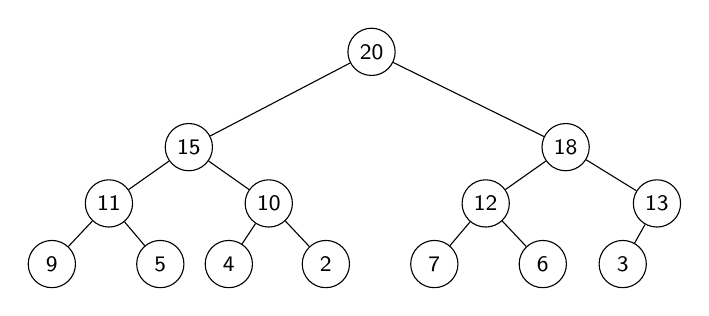
\begin{tikzpicture}[x=1.45cm,y=1.1cm,v/.style={circle,draw,inner sep=0pt,minimum size=6mm,font=\footnotesize\sffamily},s/.style={v,fill=black!25}]
\node[v] (n20) at (3.40,0) {20};
\node[v] (n18) at (5.10,-1.1) {18};
\node[v] (n15) at (1.80,-1.1) {15};
\node[v] (n13) at (5.90,-1.75) {13};
\node[v] (n12) at (4.40,-1.75) {12};
\node[v] (n10) at (2.50,-1.75) {10};
\node[v] (n11) at (1.10,-1.75) {11};
\node[v] (n3) at (5.60,-2.45) {3};
\node[v] (n6) at (4.90,-2.45) {6};
\node[v] (n7) at (3.95,-2.45) {7};
\node[v] (n2) at (3.00,-2.45) {2};
\node[v] (n4) at (2.15,-2.45) {4};
\node[v] (n5) at (1.55,-2.45) {5};
\node[v] (n9) at (0.60,-2.45) {9};
\draw (n20)--(n18) (n20)--(n15) (n18)--(n13) (n18)--(n12) (n13)--(n3) (n12)--(n6) (n12)--(n7) (n15)--(n10) (n15)--(n11) (n10)--(n2) (n10)--(n4) (n11)--(n5) (n11)--(n9);
\end{tikzpicture}
\end{center}
上圖是 \texttt{unknown(r)} 之後的樹：根 $20$ 的左子節點變成 $15$、右子節點變成 $18$，依此類推。 $13$ 只有
一個子節點 $3$，不論原圖裡 $3$ 畫在 $13$ 的左邊還是右邊，$3$ 都是 $13$ 子樹裡唯一的葉子，而 $13$ 的子樹在
鏡像裡是最右邊的那一塊，所以答案不受影響。 (A) $7$ 和 (B) $6$ 鏡像後在 $12$ 底下，排在 $3$ 的左邊；(D) $2$
在根的左半邊。
\end{pastsoln}
